\documentclass{article}
\usepackage{lipsum}
\usepackage{blindtext}

\usepackage{graphicx}
\graphicspath{ {./images/} }
\title{\LaTeX Document Template}
\date{2017-03-23}
\author{Keerthi Bandara}

\begin{document}
    \pagenumbering{gobble}
    \maketitle

% dedication
	\newpage
    \pagenumbering{roman}
    \begin{flushright}
    This latex template is dedicated to all the scientists world wide who works hard for the success of science.\\ 
    - Keerthi
    \end{flushright}
    
% abstract    
    \newpage 
	\begin{abstract}
	\blindtext
	\end{abstract}

% acknowledgements

% toc
    \newpage 
	\tableofcontents

% list of figures
	\newpage
	\listoffigures

% list of tables
	\listoftables

    
%
% Chapter 1 - Introduction
%
	\newpage
	\pagenumbering{arabic}
    \section{Introduction}
    \lipsum[2-4]
    
        \subsection{Subsection}
        \paragraph{}
        \blindtext

        \subsubsection{Subsubsection}
		\paragraph{}        
        \blindtext
        
        \paragraph{}
        \blindtext 
        
        \begin{figure}[ht]
  		\centering
    		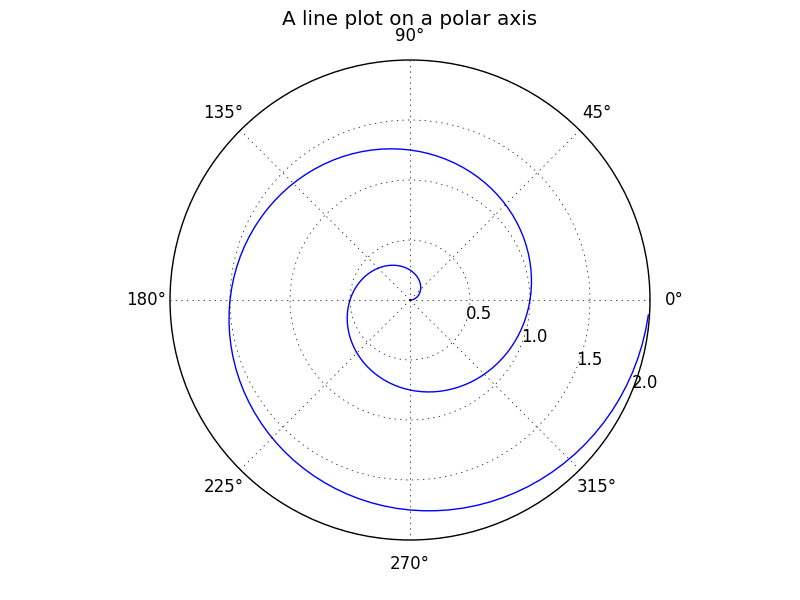
\includegraphics[scale=0.5]{./images/figure_1}
    		\caption{Polar Axis.}
		\end{figure}

        \paragraph{}
        \blindtext
        
        \begin{figure}[ht]
  		\centering
    		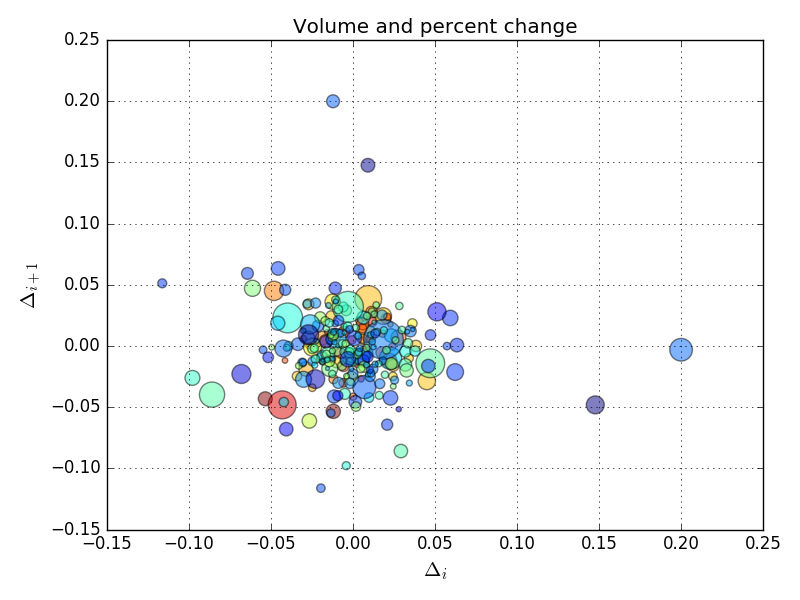
\includegraphics[scale=0.5]{./images/figure_2}
    		\caption{Scatter Plot.}
		\end{figure}
		
        \subparagraph{subparagraph}
        \blindtext
        
        \subsection{Another Subsection}
    		\blindtext

%
% Chapter 2 - Fact Finding
%    
    \newpage
    	\section{Fact Finding}
    	\paragraph{}
	This is obvious \cite{norman}.
	
	\paragraph{}
	The table \ref{table:1} is an example of referenced \LaTeX elements.
 
	\begin{table}[ht]
	\centering
	\begin{tabular}{||c c c c||} 
	\hline
	Col1 & Col2 & Col2 & Col3 \\ [0.5ex] 
	\hline\hline
	1 & 6 & 87837 & 787 \\ 
	2 & 7 & 78 & 5415 \\
	3 & 545 & 778 & 7507 \\
	4 & 545 & 18744 & 7560 \\
	5 & 88 & 788 & 6344 \\ [1ex] 
	\hline
	\end{tabular}
	\caption{Sample Data Set}
	\label{table:1}
	\end{table}

% apendices    	
    	\newpage
    	\appendix
    	\section{First Appendix}
	Text of Appendix A is Here
	
	\section{Second Appendix}
	Text of Appendix B is Here

% bibliography
	\newpage
	\begin{thebibliography}{1}
	\bibitem{notes} John W. Dower {\em Readings compiled for History 21.479.}  1991.

  \bibitem{impj}  The Japan Reader {\em Imperial Japan 1800-1945} 1973: Random House, N.Y.

  \bibitem{norman} E. H. Norman {\em Japan's emergence as a modern state} 1940: International Secretariat, Institute of Pacific Relations.

  \bibitem{fo} Bob Tadashi Wakabayashi {\em Anti-Foreignism and Western Learning in Early-Modern Japan} 1986: Harvard University Press.

  \end{thebibliography}
  

\end{document}

